\documentclass[tikz]{standalone}

\usepackage[T1]{fontenc}
\usepackage[english]{babel}

\begin{document}
	\begin{tikzpicture}
		\node[visible on=<1-2>] (dsm) at (0,0) {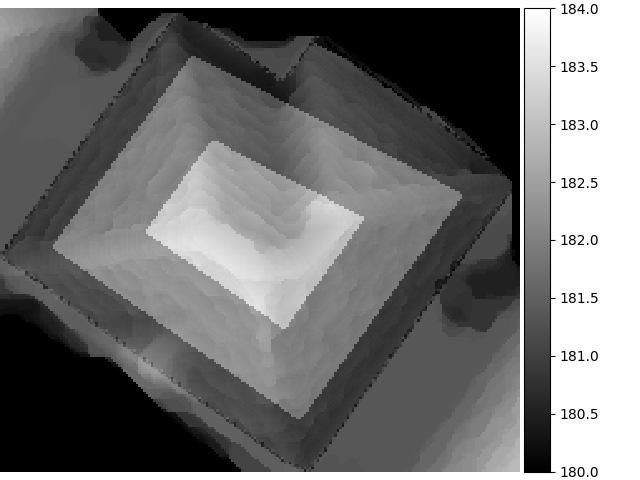
\includegraphics[width=3cm]{images/features/scatnet/dsm}};
        \path (dsm.south) node[anchor=north, text width=3cm, align=center, visible on=<1-2>] (dsm_legend) {\scriptsize \acrshort{acr::dsm}};

        \path (dsm.east) node[anchor=west, visible on=<2>] (minus) {\Large --};

		\path (minus.east) node[anchor=west, visible on=<2>] (model) {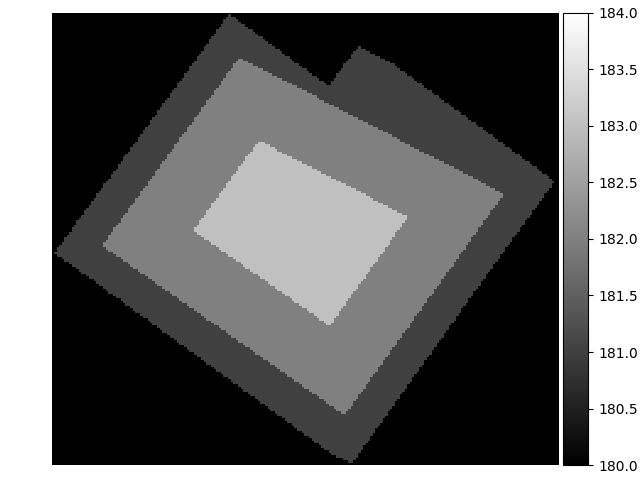
\includegraphics[width=3cm]{images/features/scatnet/height_map}};
        \path (model.south) node[anchor=north, text width=3cm, align=center, visible on=<2>] (model_legend) {\scriptsize Model heights};

        \path (minus) node[visible on=<3>] (residual_colorbar) {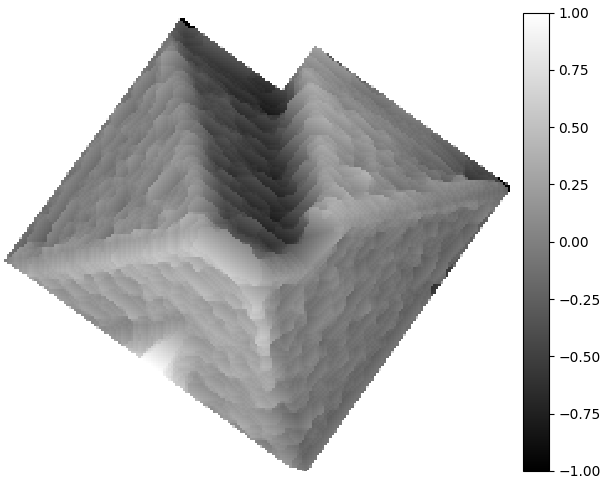
\includegraphics[width=3cm]{images/features/scatnet/residual_colbar}};
        \path (residual_colorbar.south) node[anchor=north, text width=3cm, align=center, visible on=<3>] (residual_legend) {\scriptsize Residuals};

        \path (residual_colorbar.west) node[anchor=east, visible on=<3>] (equals) {\Large =};

        \path (dsm) node[anchor=east, visible on=<4->] (residual) {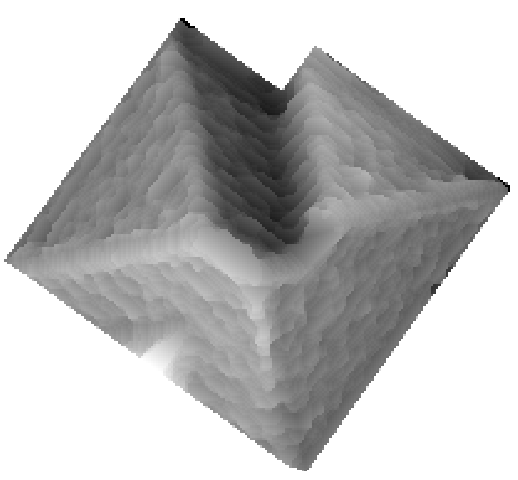
\includegraphics[width=3cm]{images/features/scatnet/residual}};
        \path (model) node[anchor=west, visible on=<4->, blue] (s) {\small \(\begin{Bmatrix}
            S_0[x](\bullet)\\
            S_1[x](\bullet, i_1, \theta_1)\\
            \vdots\\
            S_2[x](\bullet, i_1, \theta_1, i_2, \xi_2, \theta_2)\\
            \vdots
        \end{Bmatrix}\)};

        \draw[->, very thick, visible on=<4->, black] (residual) -- (s) node[pos=.15, midway, anchor=west, visible on=<4->, draw, rounded corners, black, fill=white] (scatnet) {\gls{acr::scatnet}};
	\end{tikzpicture}
\end{document}
